% =============================================================================
\section{Results}
\label{sec:results}
% =============================================================================

\subsection{Reference cohort composition changes the reported score}
\label{sec:res_cohort}

\paragraph{The default protocol selects an atypical block}
Taking the first $500$ filenames in sorted order from the BraTS slice directory
yields images from $17$ subjects. Randomly sampling $500$ slices from the same
directory spans $413$. Both satisfy a caption reading ``$N = 500$ real
slices'', and they give different answers: MMD$^2$ at \Lb{12} against the same
DDPM samples is $0.150$ for the \textsc{head} reference and $0.077$ for the
random one, a factor of $1.95$.

Subject count alone does not explain this. Table~\ref{tab:blocks} compares
$17$-subject blocks drawn from different positions in the cohort, each
supplying $500$ slices drawn identically. Every block other than the first
gives $\widehat{\mmd}^2 \approx 0.082$; the first gives $0.152$. The effect is
therefore specific to \emph{which} subjects the protocol selects, not to how
many, and it is not a sample-size artefact.

We can state what we measured but not, from this data, its cause. BraTS 2021
does not release a per-subject site label, so we cannot confirm that the
lowest-numbered subjects share a contributing institution; acquisition-site or
protocol grouping correlated with subject-identifier order is the most
economical explanation for a block-structured effect of this size, but it
remains a hypothesis. What matters for the argument here is weaker and
established directly: subject identifiers are not exchangeable, so any protocol
that selects subjects by identifier order is selecting a structured subset of
the cohort.

\begin{table}[t]
\centering
\caption{Seventeen-subject reference blocks drawn from different positions in
the BraTS subject list, each supplying $500$ slices, scored against the same
DDPM sample. Only the block that the default protocol selects is anomalous.}
\label{tab:blocks}
\begin{tabular}{lc}
\toprule
Reference block ($17$ subjects, $N = 500$) & $\widehat{\mmd}^2$ at \Lb{12} \\
\midrule
First $17$ subjects (what \textsc{head} selects) & $0.152$ \\
Middle $17$ subjects                             & $0.084$ \\
Last $17$ subjects                               & $0.082$ \\
Random $17$ subjects (seed $0$)                  & $0.081$ \\
Random $17$ subjects (seed $2$)                  & $0.082$ \\
\bottomrule
\end{tabular}
\end{table}

\paragraph{Real-versus-real distance can exceed real-versus-generated distance}
Table~\ref{tab:realreal} places that site effect on the same scale as the
quantity the metric is meant to report. Two arbitrary $17$-subject real cohorts
differ by $\widehat{\mmd}^2 = 0.017$. The first-$17$ block differs from the rest
of the real cohort by $0.096$. A subject-diverse real reference differs from
DDPM output by $0.080$. The distance between two sets of \emph{real} BraTS
images therefore exceeds the distance between real images and generated ones,
whenever one of them is the atypical block that the default reference protocol
happens to select. We stress the scope of this claim: it is
not that typical real cohort pairs exceed the generated distance --- they do
not, at $0.017$ --- but that the worst-case pair, which is the one the
convenient protocol selects, does.

\begin{table}[t]
\centering
\caption{Distances on a common scale (\Lb{12}, $N = 500$, all cohorts
$17$ subjects so that cohort size is not a confound). The third row involves no
generated images at all, yet exceeds the second.}
\label{tab:realreal}
\begin{tabular}{llc}
\toprule
Comparison & Content & $\widehat{\mmd}^2$ \\
\midrule
Real cohort A vs.\ real cohort B     & real vs.\ real      & $0.017$ \\
Real cohort A vs.\ DDPM              & real vs.\ generated & $0.080$ \\
First-$17$ block vs.\ real cohort A  & real vs.\ real      & $\mathbf{0.096}$ \\
First-$17$ block vs.\ DDPM           & real vs.\ generated & $0.152$ \\
\bottomrule
\end{tabular}
\end{table}

\paragraph{Cohort diversity mostly moves the null, not the signal}
Holding $N = 500$ fixed and sweeping the number of contributing subjects
(Table~\ref{tab:refsweep}, Fig.~\ref{fig:refsweep}) separates two effects. The
real-versus-generated distance is comparatively stable, rising by $9\%$ at
\Lb{12} between a $400$-subject and a $17$-subject reference. The
real-versus-real null is not: it rises from $0.0000$ to $0.0072$ over the same
range. FID moves more than either MMD variant, from $67.9$ to $85.3$
($1.26\times$), consistent with its estimator depending on how well the
reference covariance is estimated. The practical consequence is that reducing
cohort diversity mainly destroys the evaluator's ability to distinguish a real
cohort from a generated one, rather than changing the headline number by much
--- a failure a single reported scalar cannot expose.

\begin{table}[t]
\centering
\caption{Reference cohort diversity at fixed $N = 500$ slices, mean $\pm$ s.d.\
over three draws. Subject diversity moves the real-versus-real null far more
than it moves the real-versus-generated score.}
\label{tab:refsweep}
\begin{tabular}{rccccc}
\toprule
Subjects & $\widehat{\mmd}^2$ \Lb{8} & $\widehat{\mmd}^2$ \Lb{12}
         & null \Lb{8} & null \Lb{12} & FID \\
\midrule
$17$  & $0.1021 \pm 0.0046$ & $0.0801 \pm 0.0030$ & $0.0082$ & $0.0072$ & $85.3 \pm 1.8$ \\
$25$  & $0.1026 \pm 0.0037$ & $0.0799 \pm 0.0025$ & $0.0088$ & $0.0074$ & $82.8 \pm 1.6$ \\
$50$  & $0.0975 \pm 0.0035$ & $0.0751 \pm 0.0026$ & $0.0024$ & $0.0024$ & $71.7 \pm 1.0$ \\
$100$ & $0.0958 \pm 0.0016$ & $0.0739 \pm 0.0005$ & $0.0011$ & $0.0010$ & $72.5 \pm 0.4$ \\
$200$ & $0.0966 \pm 0.0032$ & $0.0749 \pm 0.0023$ & $0.0003$ & $0.0002$ & $68.4 \pm 0.6$ \\
$400$ & $0.0957 \pm 0.0013$ & $0.0736 \pm 0.0008$ & $0.0000$ & $0.0000$ & $67.9 \pm 0.4$ \\
\midrule
$400 \rightarrow 17$ & $\times 1.07$ & $\times 1.09$
  & $+0.0082$ & $+0.0072$ & $\times 1.26$ \\
\bottomrule
\end{tabular}
\end{table}

\begin{figure}[t]
\centering
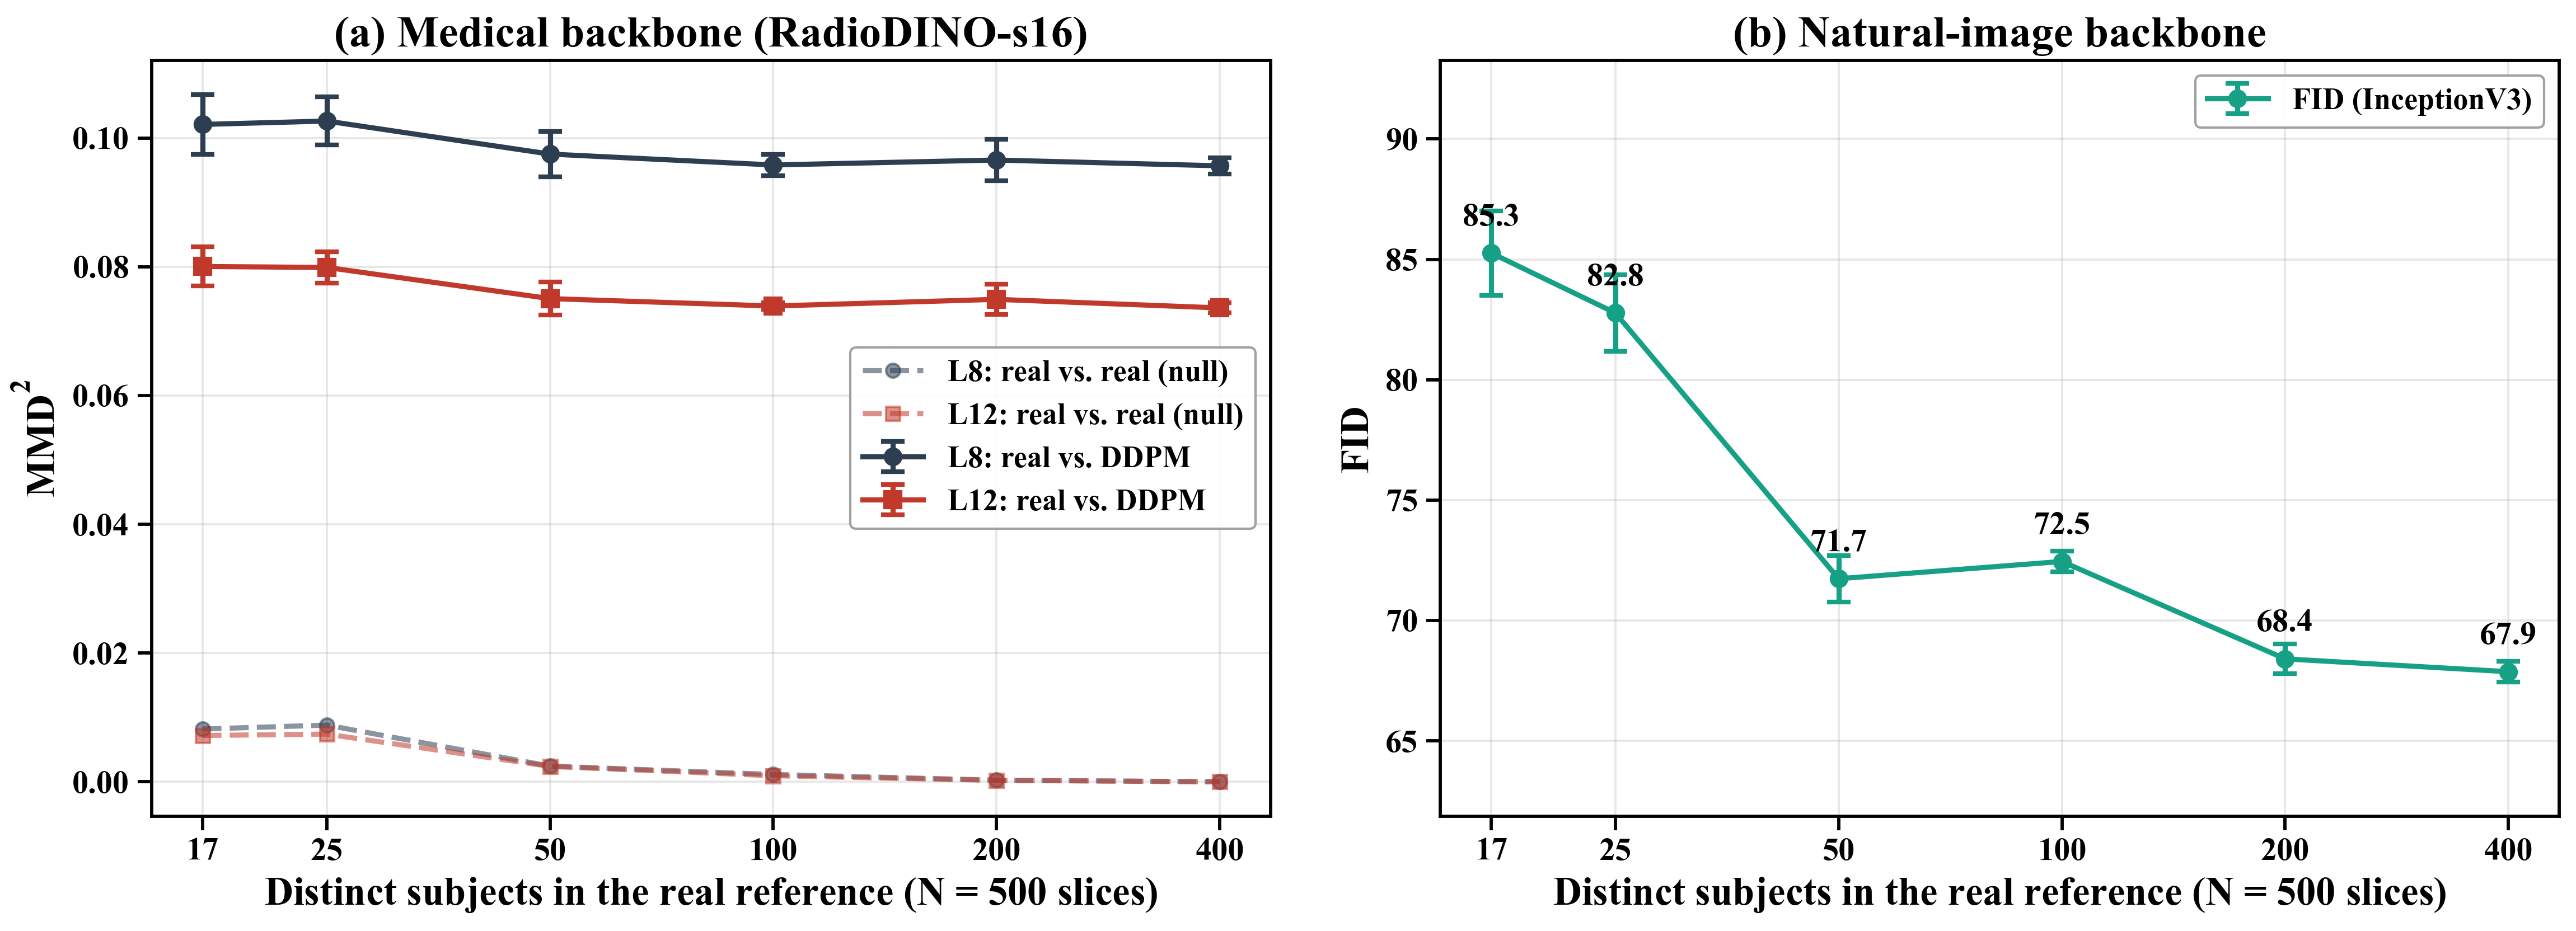
\includegraphics[width=\linewidth]{Images/reference_set_construction.png}
\caption{Reference cohort diversity at fixed $N = 500$. (a) RadioDINO-s16
MMD$^2$ against DDPM output (solid) and against a held-out real probe
(dashed). The generated distance is comparatively flat, whereas the
real-versus-real null grows sharply as diversity falls. (b) FID on the same
references.}
\label{fig:refsweep}
\end{figure}

\subsection{An empirical inter-cohort reference distribution}
\label{sec:res_null}

Table~\ref{tab:cohortnull} reports the null of Eq.~\eqref{eq:null} at three
cohort sizes, together with each generator's position within it. Two
observations follow.

First, the permutation test does not discriminate here. It assigns $z > 340$ and
$\hat{p}$ at the resolution floor to every generator at every cohort size,
including generators as different from one another as a fine-tuned in-domain
DDPM and colour fundus photography. It answers a question whose answer was
never in doubt.

Second, and more revealing, the two nulls move in \emph{opposite} directions as
the reference improves. Going from a $17$- to a $100$-subject reference, the
inter-cohort statistic for the DDPM rises from $z_{\mathrm{cohort}} = 15.7$
to $89.0$, correctly reporting that a more representative reference resolves
the generator gap more sharply. Over the same range the permutation statistic
\emph{falls}, from $z = 423$ to $z = 347$. The permutation null is built by
shuffling labels within the pooled sample, so a more heterogeneous real set
inflates the null variance and depresses the statistic: a better reference
makes the conventional test report less significance. The inter-cohort reference
distribution does not have this defect, because it is constructed from real
cohorts only.

For an interpretable effect size we report the generator distance as a multiple
of the \emph{mean} real-versus-real cohort distance. With a $17$-subject
reference the DDPM sits at $5.5\times$ the mean real cohort pair; at $50$
subjects, $14.5\times$; at $100$ subjects, $30.3\times$.

We use the mean rather than the maximum deliberately. A ratio to the largest
observed cohort distance is a ratio to an order statistic, whose expectation
grows with the number of pairs compared, so it is not comparable across
conditions that contribute different numbers of pairs. Our $17$- and
$50$-subject conditions both use $K = 24$ blocks and therefore exactly $276$
pairs, and the effect is already established between them with the pair count
held fixed: the ratio to the mean rises from $5.5\times$ to $14.5\times$, and
the ratio to the maximum from $2.3\times$ to $6.9\times$. The $100$-subject
condition admits only $K = 12$ disjoint blocks at this cohort size and so rests
on $66$ pairs; its maximum is drawn from a smaller sample and we do not compare
it to the others on that basis. Table~\ref{tab:cohortnull} reports the mean,
the $95$th percentile and the maximum so the reader can apply whichever
summary they prefer.

\begin{table}[t]
\centering
\caption{Inter-cohort reference distribution at \Lb{12} and generator positions
within it. $z_{\mathrm{cohort}}$ rises with a better reference; the permutation
$z$ falls. ``$\times$mean'' and ``$\times$max'' are the generator distance as a
multiple of the mean and the largest real-versus-real cohort distance; the
former is preferred because the latter is an order statistic whose expectation
depends on the number of pairs. The $17$- and $50$-subject rows rest on the
same $K = 24$ blocks and $276$ pairs and are directly comparable; the
$100$-subject rows rest on $66$ pairs.}
\label{tab:cohortnull}
\small
\begin{tabular}{llcccccc}
\toprule
Cohort & Set & $\widehat{\mmd}^2$ & $\times$mean & $\times$max
 & $z_{\mathrm{cohort}}$ & $z_{\mathrm{perm}}$ & $\hat{p}_{\mathrm{perm}}$ \\
\midrule
\multirow{5}{*}{\shortstack[l]{$17$ subj.\\$K=24$}}
 & null ($276$ pairs) & $0.017 \pm 0.005$ & --- & --- & --- & --- & --- \\
 & DDPM      & $0.095$ & $5.5$  & $2.3$  & $15.7$ & $423.3$ & $<0.002$ \\
 & WDM-3D    & $0.225$ & $13.0$ & $5.5$  & $42.0$ & $709.2$ & $<0.002$ \\
 & LIDC CT   & $0.410$ & $23.6$ & $10.1$ & $79.3$ & $719.1$ & $<0.002$ \\
 & Retinal   & $0.475$ & $27.4$ & $11.7$ & $92.4$ & $810.2$ & $<0.002$ \\
\midrule
\multirow{5}{*}{\shortstack[l]{$50$ subj.\\$K=24$}}
 & null ($276$ pairs) & $0.006 \pm 0.002$ & --- & --- & --- & --- & --- \\
 & DDPM      & $0.081$ & $14.5$ & $6.9$  & $49.5$  & $381.6$ & $<0.002$ \\
 & WDM-3D    & $0.216$ & $38.8$ & $18.5$ & $138.7$ & $689.4$ & $<0.002$ \\
 & LIDC CT   & $0.402$ & $72.2$ & $34.4$ & $261.0$ & $711.1$ & $<0.002$ \\
 & Retinal   & $0.461$ & $82.7$ & $39.4$ & $299.4$ & $810.4$ & $<0.002$ \\
\midrule
\multirow{5}{*}{\shortstack[l]{$100$ subj.\\$K=12$}}
 & null ($66$ pairs) & $0.003 \pm 0.001$ & --- & --- & --- & --- & --- \\
 & DDPM      & $0.079$ & $30.3$  & $15.9$ & $89.0$  & $347.2$ & $<0.002$ \\
 & WDM-3D    & $0.220$ & $84.3$  & $44.1$ & $253.3$ & $631.4$ & $<0.002$ \\
 & LIDC CT   & $0.403$ & $154.4$ & $80.8$ & $466.0$ & $678.3$ & $<0.002$ \\
 & Retinal   & $0.463$ & $177.2$ & $92.7$ & $535.6$ & $766.2$ & $<0.002$ \\
\bottomrule
\end{tabular}
\end{table}

\begin{figure}[t]
\centering
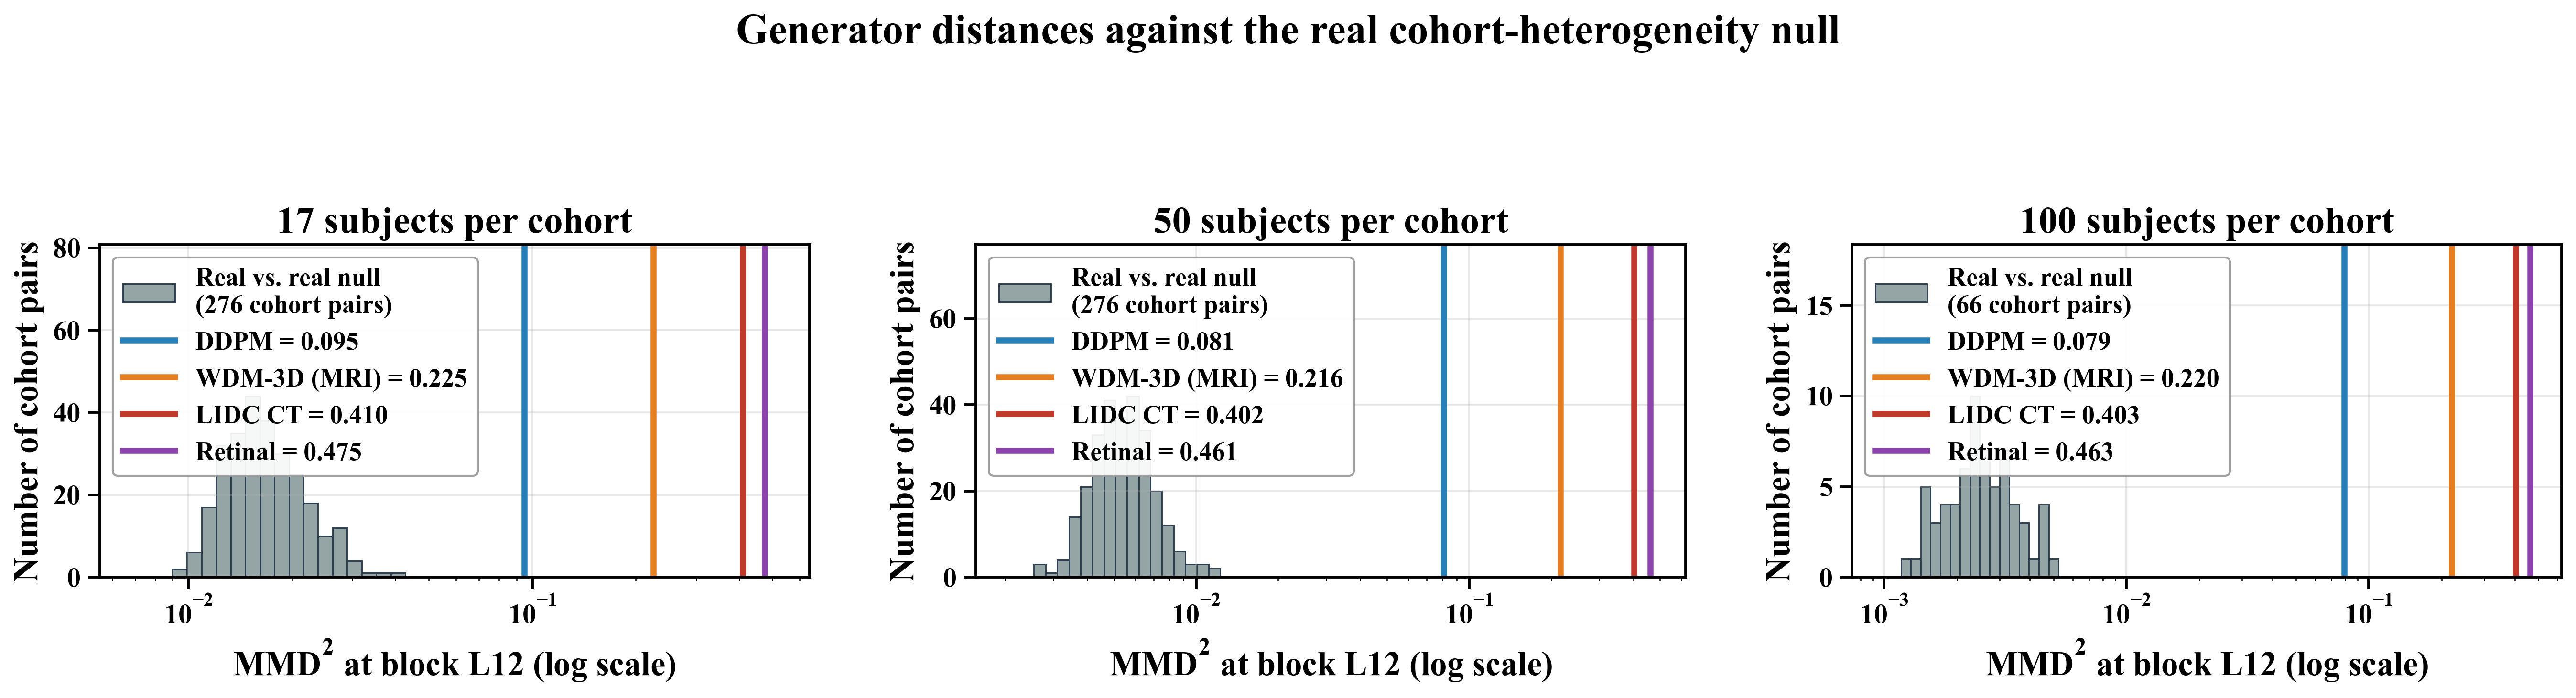
\includegraphics[width=\linewidth]{Images/cohort_heterogeneity_null.png}
\caption{Generator distances against the real cohort-heterogeneity null at
three cohort sizes. Histograms are pairwise distances between disjoint real
patient blocks; vertical lines mark generators. The horizontal axis is
logarithmic, because the null lies roughly two orders of magnitude below the
generator distances and is not visible on a linear scale. As cohorts grow the
null shifts left and concentrates, while the generator distances stay
essentially fixed --- the separation the evaluation can resolve is set by the
reference, not by the generators.}
\label{fig:cohortnull}
\end{figure}
